\chapter{Specifikacija programske potpore}
		
	\section{Funkcionalni zahtjevi}
			
			\noindent \textbf{Dionici:}
			
			\begin{packed_enum}
				
				\item Klijent
				\item Registrirani korisnik/Ponuditelj		
				\begin{packed_enum}
                    				\item Izdavač
                    				\item Preprodavač
                   				\item Antikvarijat
                			\end{packed_enum}
                			\item Strani izdavač
                			\item Razvojni tim
			\end{packed_enum}
			
			\noindent \textbf{Akteri i njihovi funkcionalni zahtjevi:}
			
			
			\begin{packed_enum}

				 \item \underbar{Neregistrirani ili registrirani korisnik može:}
                
   				\begin{packed_enum}
       				\item Pretraživati knjige po njihovim atributima i po ponuditeljima
       				\item Pregledavati objave
       				\item Pristupiti profilu ponuditelja
			      	\item Pretraživati na karti ponuditelje                      				
                  				\end{packed_enum}
				\item  \underbar{Neregistrirani korisnik (inicijator) može:}
				
				\begin{packed_enum}
					\item Napraviti korisnički račun registracijom za što mu treba korisničko ime, naziv, lozinka, e-mail, broj mobitela i adresa i može birati u koju će kategoriju ponuditelja spadati
					\item Slati zahtjev izdavačima da se knjiga na stranom jeziku prevede		
				\end{packed_enum}
			
				\item  \underbar{Registrirani korisnik tj. ponuditelj (izdavač/antikvarijat/preprodavač)(inicijator) može:} %bilo bi pozeljno za svaku vrstu reg korisnika napisati sto moze?
				
				\begin{packed_enum}
					
					\item Prijaviti se u sustav koristeći korisničko ime i lozinku
                   				\item Pregledavati svoj račun, mijenjati njegove podatke i izbrisati ga
					\item Stavljati , mijenjati i brisati njegove objave za knjige
					
				\end{packed_enum}

				\item \underbar{Izdavač (inicijator) može:}

                				\begin{packed_enum}
                    					\item Slati zahtjev za prijevod knjige stranom izdavaču
                				\end{packed_enum}

                			\item \underbar{Administrator(sudionik):}
                			\begin{packed_enum}
                    				\item Prima zahtjev za registraciju i na temelju unesenih podataka potvrđuje ili odbija registraciju
                			\end{packed_enum}

                			\item \underbar{Strani izdavač(sudionik):}
                			\begin{packed_enum}
                    				\item Prima zahtjev od strane izdavača za prijevod knjige
                			\end{packed_enum}

                			\item \underbar{Baza podataka(sudionik):}
                			\begin{packed_enum}
                    				\item Pohranjuje podatke o korisnicima i njihovim ovlastima
                    				\item Pohranjuje podatke o objavljenim knjigama
					\item Pohranjuje podatke o zahtjevima
                			\end{packed_enum}
			\end{packed_enum}
			
			\eject 
			
			
			\subsection{Obrasci uporabe}
				

				
				\subsubsection{Opis obrazaca uporabe}				
					\noindent \underbar{\textbf{UC1 - Registracija}}
            
					\begin{packed_item}

						\item  \textbf{Glavni sudionik: } Neregistrirani korisnik
						\item  \textbf{Cilj:} Izrada korisničkog računa za web stranicu
						\item  \textbf{Sudionici:} Baza podataka
						\item  \textbf{Preduvjet:} Pristup aplikaciji
						\item  \textbf{Opis osnovnog tijeka:}
						
						\item[] \begin{packed_enum}
	
							\item Neregistrirani korisnik bira opciju registracije
                           					\item Unosi podatke potrebne za registraciju
							\item Web obavještava korisnika da će zahtjev za registraciju pregledati administrator
						\end{packed_enum}
						
						\item  \textbf{Opis mogućih odstupanja:}
						
						\item[] \begin{packed_item}
	
							\item[2.a] Korisnik unosi zauzeto korisničko ime, e-mail ili broj telefona ili je neki od podataka u krivom formatu
							\item[] \begin{packed_enum}
								
								\item Sustav obavještava o neuspjeloj registraciji i gdje je došlo do greške
								\item Korisnik unosi prihvatljive podatke ili odustane od registracije
								
							\end{packed_enum}
						\end{packed_item}
					\end{packed_item}

                    \noindent \underbar{\textbf{UC2- Prijava}}
					\begin{packed_item}
	
						\item \textbf{Glavni sudionik: } Ponuditelj
						\item  \textbf{Cilj:} Dobiti pristup web stranici sa postojećim korisničkim računom
						\item  \textbf{Sudionici:} Baza podataka
						\item  \textbf{Preduvjet:} - Ponuditelj ima izrađen korisnički račun
						\item  \textbf{Opis osnovnog tijeka:}
						
						\item[] \begin{packed_enum}	
							\item Ponuditelj bira opciju prijave
							\item Ponuditelj unosi korisničko ime i lozinku
                            					\item Ponuditelj dobiva pristup svom korisničkom računu
						\end{packed_enum}
						
						\item  \textbf{Opis mogućih odstupanja:}
						
						\item[] \begin{packed_item}
	
							\item[2.a] Jedan ili više potrebnih podataka je krivo uneseno
							\item[] \begin{packed_enum}
								
								\item Sustav obavještava o neuspjeloj prijavi i gdje je došlo do greške
								\item Ponuditelj unosi prihvatljive podatke ili odustane od prijave
								
							\end{packed_enum}
						\end{packed_item}
					\end{packed_item}

                    \noindent \underbar{\textbf{UC3 - Potvrda registracije}}
					\begin{packed_item}
	
						\item \textbf{Glavni sudionik: } Administrator
						\item  \textbf{Cilj:} Potvrđivanje uspješne/neuspješne registracije ponuditelja
						\item  \textbf{Sudionici:} Baza podataka, neregistrirani korisnik
						\item  \textbf{Preduvjet:} - Neregistrirani korisnik pokušava izvršiti registraciju
						\item  \textbf{Opis osnovnog tijeka:}
						
						\item[] \begin{packed_enum}	
							\item Nakon što korisnik unese podatke za registraciju, zahtjev za registraciju se šalje administratoru na pregled
							\item Provjerava se da su uneseni podaci dobrog oblika i da ne postoje u bazi podataka
                           					\item Administrator potvrđuje unesene podatke i informira da je registracija uspješna
						\end{packed_enum}
						
						\item  \textbf{Opis mogućih odstupanja:}
						
						\item[] \begin{packed_item}
	
							\item[2.a] Podaci su krivog formata ili već upisani u bazu podataka jer ih netko drugi koristi
							\item[] \begin{packed_enum}			
								\item Administrator obavještava da je došlo do greške i zašto
							\end{packed_enum}
						\end{packed_item}
					\end{packed_item}

                    \noindent \underbar{\textbf{UC4 - Biranje kategorije ponuditelja}}
					\begin{packed_item}
	
						\item \textbf{Glavni sudionik: } Neregistrirani korisnik
						\item  \textbf{Cilj:} Biranje kategorije ponuditelja u koju će spadati korisnički račun
						\item  \textbf{Sudionici:} Baza podataka
						\item  \textbf{Preduvjet:} - Korisnik je započeo registraciju
						\item  \textbf{Opis osnovnog tijeka:}
						
						\item[] \begin{packed_enum}
	
							\item Pri registraciji korisnik klikne na polje kojim bira u koju će kategoriju spadati
							\item Korisnik bira kategoriju i nastavlja sa registracijom
						\end{packed_enum}
						
						\item  \textbf{Opis mogućih odstupanja:-}
					
					\end{packed_item}

                    \noindent \underbar{\textbf{UC5 - Pregled korisničkog računa}}
					\begin{packed_item}
	
						\item \textbf{Glavni sudionik: } Ponuditelj
						\item  \textbf{Cilj:} Ponuditelj pregledava podatke o svom korisničkom računu
						\item  \textbf{Sudionici:} Baza podataka
						\item  \textbf{Preduvjet:} - Ponuditelj je prijavljen
						\item  \textbf{Opis osnovnog tijeka:}
						
						\item[] \begin{packed_enum}
	
							\item Ponuditelj bira opciju "Moj račun"
							\item Aplikacija prikazuje pripadni korisnički račun i podatke
						\end{packed_enum}
						
						\item  \textbf{Opis mogućih odstupanja: -}
						
					\end{packed_item}

                    \noindent \underbar{\textbf{UC6 - Dodavanje objave}}
					\begin{packed_item}
	
						\item \textbf{Glavni sudionik: } Ponuditelj
						\item  \textbf{Cilj:} Dodavanje objave knjige za prodaju na web stranicu
						\item  \textbf{Sudionici:} Baza podataka
						\item  \textbf{Preduvjet:} - Ponuditelj je prijavljen
						\item  \textbf{Opis osnovnog tijeka:}
						
						\item[] \begin{packed_enum}
	
							\item Ponuditelj bira opciju "Nova objava"
                            					\item Aplikacija otvara stranicu za novu objavu
                            					\item Ponuditelj unosi potrebne podatke
							\item Ponuditelj klikne opciju "Objavi"
                            					\item Objava knjige je vidljiva na web stranici i u bazi podataka
						\end{packed_enum}
						
						\item  \textbf{Opis mogućih odstupanja:}
						
						\item[] \begin{packed_item}
	
							\item[2.a] Ponuditelj unosi krivi format podataka potrebnih za objavu
							\item[] \begin{packed_enum}
								
								\item Aplikacija obavještava da je format kriv i gdje
								\item Ponuditelj unosi prihvatljive podatke ili odustaje od objave
							\end{packed_enum}
                            					\item[2.b] Ponuditelj ne unosi sve potrebne podatke da se napravi objava
                             					\item[] \begin{packed_enum}
                                 					\item Aplikacija obavještava da jedno ili više polja nije popunjeno
                                 					\item Ponuditelj popunjuje prazna polja ili odustaje od objave
                             					\end{packed_enum}
						\end{packed_item}
					\end{packed_item}

                    \noindent \underbar{\textbf{UC7 - Mijenjanje objave}}
					\begin{packed_item}
	
						\item \textbf{Glavni sudionik: } Ponuditelj
						\item  \textbf{Cilj:} Mijenjanje podataka objave za knjigu
						\item  \textbf{Sudionici:} Baza podataka
						\item  \textbf{Preduvjet:} - Postoji objava za knjigu
						\item  \textbf{Opis osnovnog tijeka:}
						
						\item[] \begin{packed_enum}	
							\item Ponuditelj klikne na objavu koju želi promijeniti
                            					\item Aplikacija otvara stranicu objave
							\item Ponuditelj bira opciju mijenjanja podataka
                            					\item Ponuditelj izmjenjuje podatke
                            					\item Ponuditelj sprema izmjene
                            					\item Novi podaci su zapisani u bazu podataka
						\end{packed_enum}
						
						\item  \textbf{Opis mogućih odstupanja:}
						
						\item[] \begin{packed_item}
	
							\item[2.a] Ponuditelj unosi podatke u krivom formatu
							\item[] \begin{packed_enum}
								
								\item Aplikacija obavještava gdje je došlo do greške i zašto
								\item Ponuditelj unosi prihvatljive podatke ili odustane od izmjene podataka
								
							\end{packed_enum}

                            					\item[2.b] Ponuditelj ne sprema izmjene
                            					\item[] \begin{packed_enum}
                                					\item Aplikacija obavještava da promjene nisu pohranjene	
                            					\end{packed_enum}
						\end{packed_item}
					\end{packed_item}

                    \noindent \underbar{\textbf{UC8 - Brisanje objave}}
					\begin{packed_item}
	
						\item \textbf{Glavni sudionik: } Ponuditelj
						\item  \textbf{Cilj:} Ponuditelj briše svoju objavu
						\item  \textbf{Sudionici:} Baza podataka
						\item  \textbf{Preduvjet:} - Ponuditelj ima objavu
						\item  \textbf{Opis osnovnog tijeka:}
						
						\item[] \begin{packed_enum}
	
							\item Ponuditelj klikne na svoju objavu koju želi izbrisati
                            					\item Ponuditelj bira opciju brisanja objave
							\item Aplikacija pita za potvrdu brisanja
                            					\item Ponuditelj potvrđuje
                            					\item Briše se objava iz baze podataka
						\end{packed_enum}
						
						\item  \textbf{Opis mogućih odstupanja: -}
					\end{packed_item}

                    \noindent \underbar{\textbf{UC9 - Pregled objave}}
					\begin{packed_item}
	
						\item \textbf{Glavni sudionik: } Korisnik (registrirani i neregistrirani)
						\item  \textbf{Cilj:} Pregledavanje objave za knjigu
						\item  \textbf{Sudionici:} Baza podataka, ponuditelj
						\item  \textbf{Preduvjet:} - Ponuditelj ima objavu knjige
						\item  \textbf{Opis osnovnog tijeka:}
						
						\item[] \begin{packed_enum}	
							\item Korisnik klikne na objavu
                            					\item Aplikacija prikazuje objavu i podatke o objavi
						\end{packed_enum}
						
						\item  \textbf{Opis mogućih odstupanja: -}
					\end{packed_item}

                    \noindent \underbar{\textbf{UC10 - Pregled profila ponuditelja}}
					\begin{packed_item}
	
						\item \textbf{Glavni sudionik: } Korisnik
						\item  \textbf{Cilj:} Korisnik pregledava korisnički račun nekog ponuditelja
						\item  \textbf{Sudionici:} Baza podataka
						\item  \textbf{Preduvjet:} - Ponuditelj ima izrađen korisnički račun
						\item  \textbf{Opis osnovnog tijeka:}
						
						\item[] \begin{packed_enum}
	
							\item Korisnik klikne na opciju pregledavanja korisničkog računa ponuditelja
                            					\item Aplikacija otvara stranicu na kojoj prikazuje podatke o korisničkom računu ponuditelja
						\end{packed_enum}
						
						\item  \textbf{Opis mogućih odstupanja: -}
					\end{packed_item}

                    \noindent \underbar{\textbf{UC11 - Zahtjev od neregistriranog korisnika da se knjiga prevede}}
					\begin{packed_item}
	
						\item \textbf{Glavni sudionik: } Neregistrirani korisnik
						\item  \textbf{Cilj:} Neregistrirani korisnik traži izdavača da se knjiga prevede
						\item  \textbf{Sudionici:} Baza podataka, izdavač
						\item  \textbf{Preduvjet:} - Postoji objava za knjigu
						\item  \textbf{Opis osnovnog tijeka:}
						
						\item[] \begin{packed_enum}
	
							\item Korisnik klikne na objavu za knjigu
                            					\item Aplikacija otvara stranicu objave 
							\item Korisnik klikne na opciju "Zatraži prijevod knjige"
                            					\item U bazi podataka se povećava broj zatraženih prijevoda od neregistriranih korisnika za tu knjigu
						\end{packed_enum}
						
						\item  \textbf{Opis mogućih odstupanja: -}
					\end{packed_item}

                    \noindent \underbar{\textbf{UC12 - Zahtjev stranom izdavaču za prijevod knjige}}
					\begin{packed_item}
	
						\item \textbf{Glavni sudionik: } Izdavač
						\item  \textbf{Cilj:} Izdavač šalje zahtjev stranom izdavaču da se knjiga prevede
						\item  \textbf{Sudionici:} Baza podataka, strani izdavač
						\item  \textbf{Preduvjet:} Postoji objava za knjigu
						\item  \textbf{Opis osnovnog tijeka:}
						
						\item[] \begin{packed_enum}
	
							\item Ponuditelj na svojoj objavi klikne opciju "Zatraži stranog izdavača za prijevod"
                            					\item U bazi podataka se povećava broj zatraženih prijevoda od strane izdavača
						\end{packed_enum}
						
						\item  \textbf{Opis mogućih odstupanja: -}
					\end{packed_item}

                    \noindent \underbar{\textbf{UC13 - Pretraživanje po lokaciji}}
					\begin{packed_item}
	
						\item \textbf{Glavni sudionik: } Korisnik
						\item  \textbf{Cilj:} Pretraživanje ponuditelja na mapi koristeći objavljene lokacije
						\item  \textbf{Sudionici:} Baza podataka, ponuditelj
						\item  \textbf{Preduvjet:} - Ponuditelj ima objavljenu lokaciju
						\item  \textbf{Opis osnovnog tijeka:}
						
						\item[] \begin{packed_enum}	
							\item Na glavnoj stranici je karta na kojoj se vide označene adrese ponuditelja
                            					\item Korisnik može biranjem lokacije vidjeti ponuditelja/e koji se tamo nalaze
						\end{packed_enum}
						
						\item  \textbf{Opis mogućih odstupanja: -}
					\end{packed_item}

                    \noindent \underbar{\textbf{UC14 - Detaljna pretraga objava}}
					\begin{packed_item}
	
						\item \textbf{Glavni sudionik: } Korisnik
						\item  \textbf{Cilj:} Pretraživanje objava knjiga po atributima i imenu ponuditelja
						\item  \textbf{Sudionici:} Baza podataka
						\item  \textbf{Preduvjet:} - 
						\item  \textbf{Opis osnovnog tijeka:}
						
						\item[] \begin{packed_enum}
	
							\item Korisnik klikne na opciju pretraživanja objava
							\item Korisnik ispunjava barem jedno od sljedećih polja za detaljniju pretragu: naziv knjige, naziv autora, cijena(od/do), , godina izdanja(od/do), redni broj izdanja, kategorija izdavača, žanr, ISBN, oznaka vrste knjige i ime ponuditelja
                            					\item Stranica izbacuje knjige koje se poklapaju sa upisanim karakteristikama
						\end{packed_enum}
						
						\item  \textbf{Opis mogućih odstupanja: }
						
						\item[] \begin{packed_item}
	
							\item[2.a] Ne postoji objava koja ispunjuje kriterije
							\item[] \begin{packed_enum}
								
								\item Aplikacija ne prikazuje niti jednu objavu s tekstom koij obavještava da nema objava sa danim atributima 
							\end{packed_enum}
                            					
						\end{packed_item}
					\end{packed_item}

				\eject	
				
				\subsubsection{Dijagrami obrazaca uporabe}
					
				\begin{figure}[H]
    					\centering
    					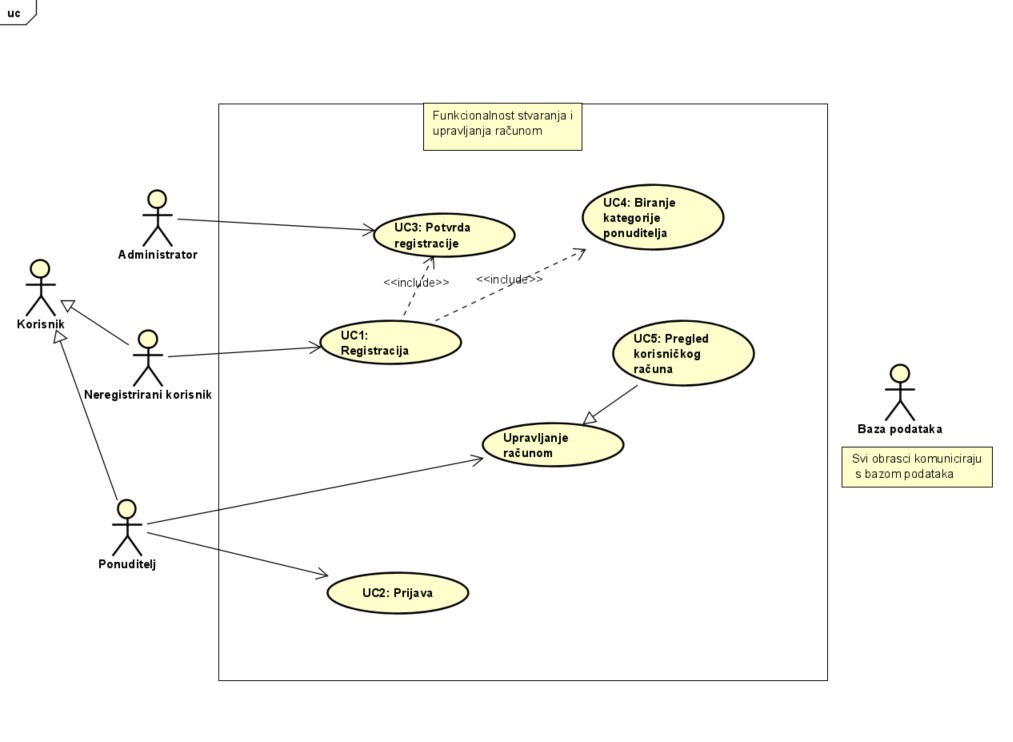
\includegraphics[width = \textwidth]{slike/DO1}
    					\caption{Dijagram obrazaca 1}
    					\label{fig:Dijagram obrazaca 1}
				\end{figure}

				\begin{figure}
    					\centering
    					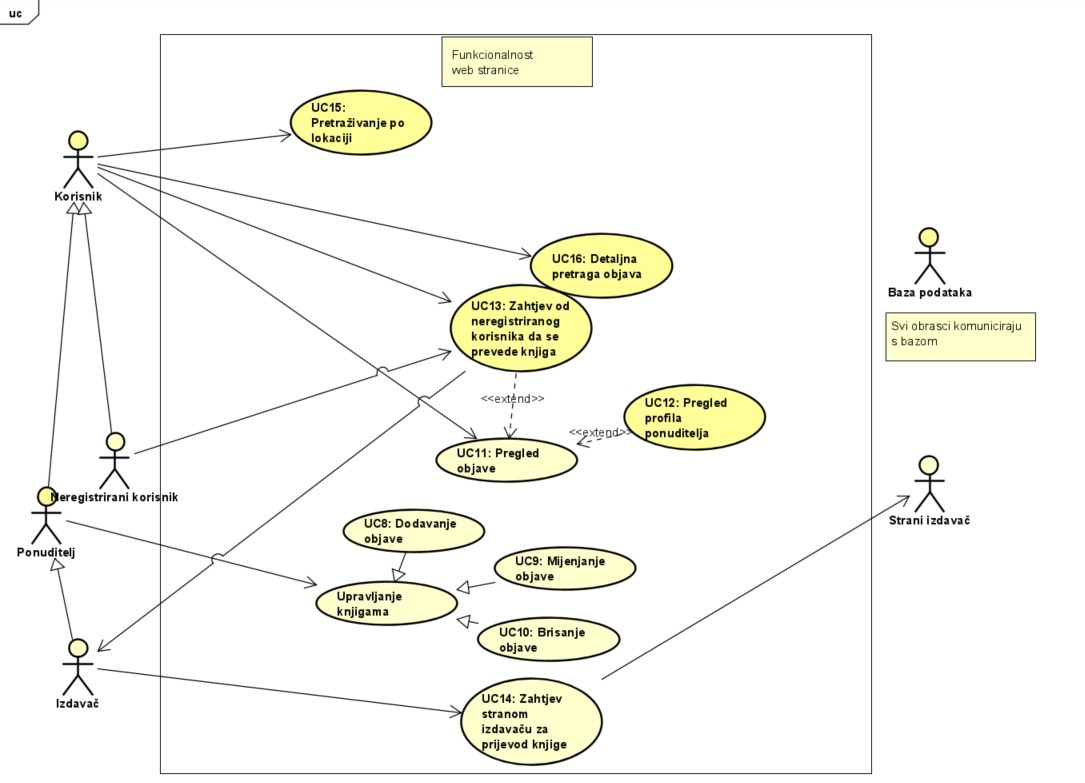
\includegraphics[width = \textwidth]{slike/DO2}
    					\caption{Dijagram obrazaca 2}
    					\label{fig:Dijagram obrazaca 2}
				\end{figure}
				\eject	
					
	
				
			\subsection{Sekvencijski dijagrami}
				
				\textbf{Obrazac uporabe UC13 – Pretraživanje po lokaciji i UC11 – Zahtjev da se prevede knjiga}\\\\
				Neregistrirani korisnik šalje zahtjev za pregled karte ponuditelja knjiga. Poslužitelj dohvaća ponuditelje knjiga iz baze i vraća prikaz karte sa označenim adresama ponuditelja. Korisnik odabire ponuditelja koji je izdavač. Poslužitelj dohvaća podatke o odabranom ponuditelju iz baze. Vraća korisniku listu svih knjiga dotičnog ponuditelja. Korisnik dodatno filtrira ponudu knjiga po želji. Korisnik traži prijevod od izdavača. U bazi podataka povećava se broj zatraženih prijevoda za tu knjigu.\\
				
				\begin{figure}[h]
					\centering
					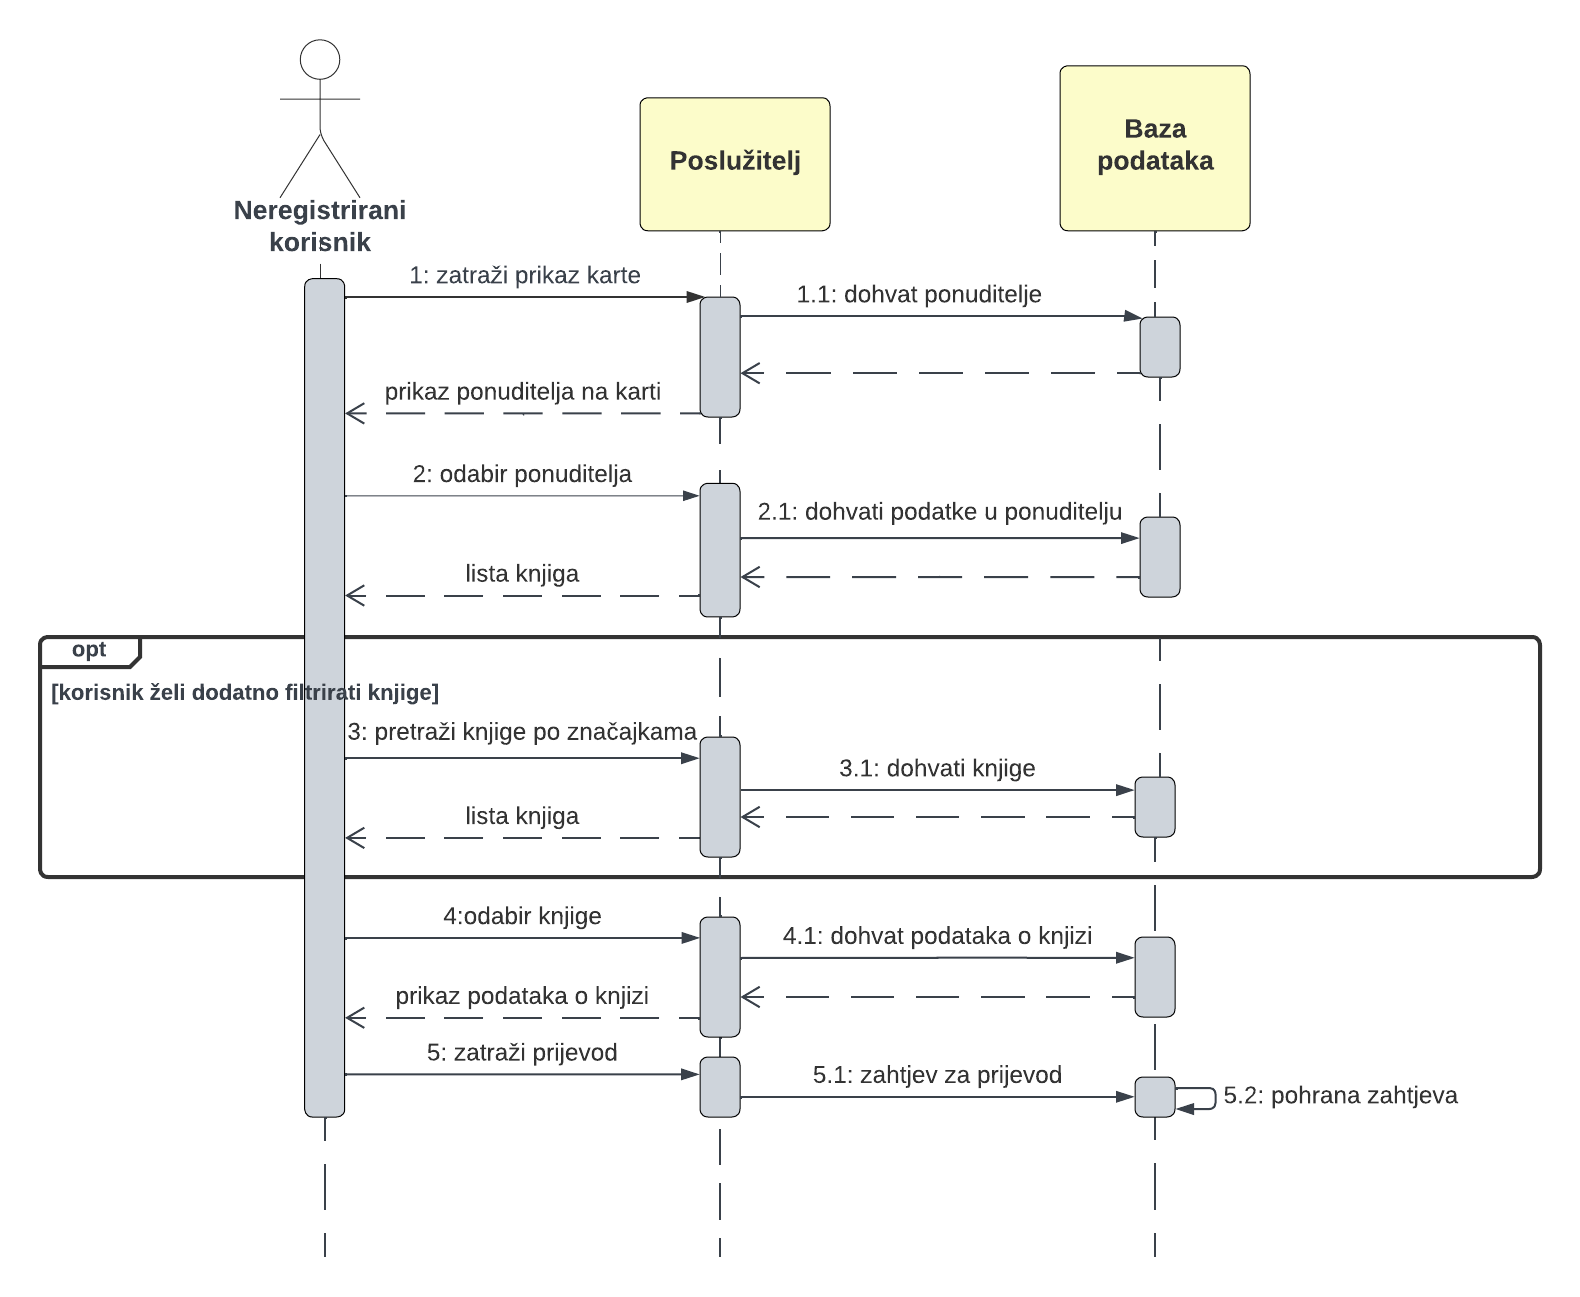
\includegraphics[width = \textwidth]{slike/sekvUC15UC13.PNG}
					\caption{Sekvencijski dijagram obrazaca uporabe UC13 i UC15}
					\label{fig:enter-label}
				\end{figure}
				\eject
				
				\textbf{Obrazac uporabe UC1 – Registracija i UC3 – Potvrda registracije}\\\\
				Neregistrirani korisnik šalje zahtjev za registraciju. Poslužitelj mu vraća formu za registraciju. Nakon što neregistrirani korisnik unese potrebne podatke za registraciju, poslužitelj ga obavještava da će administrator pregledati njegove podatke i šalje ih administratoru. Ako administrator utvrdi da je sve u redu, obavještava neregistriranog korisnika da je uspješno registriran.\\
				
				\begin{figure}[h]
					\centering
					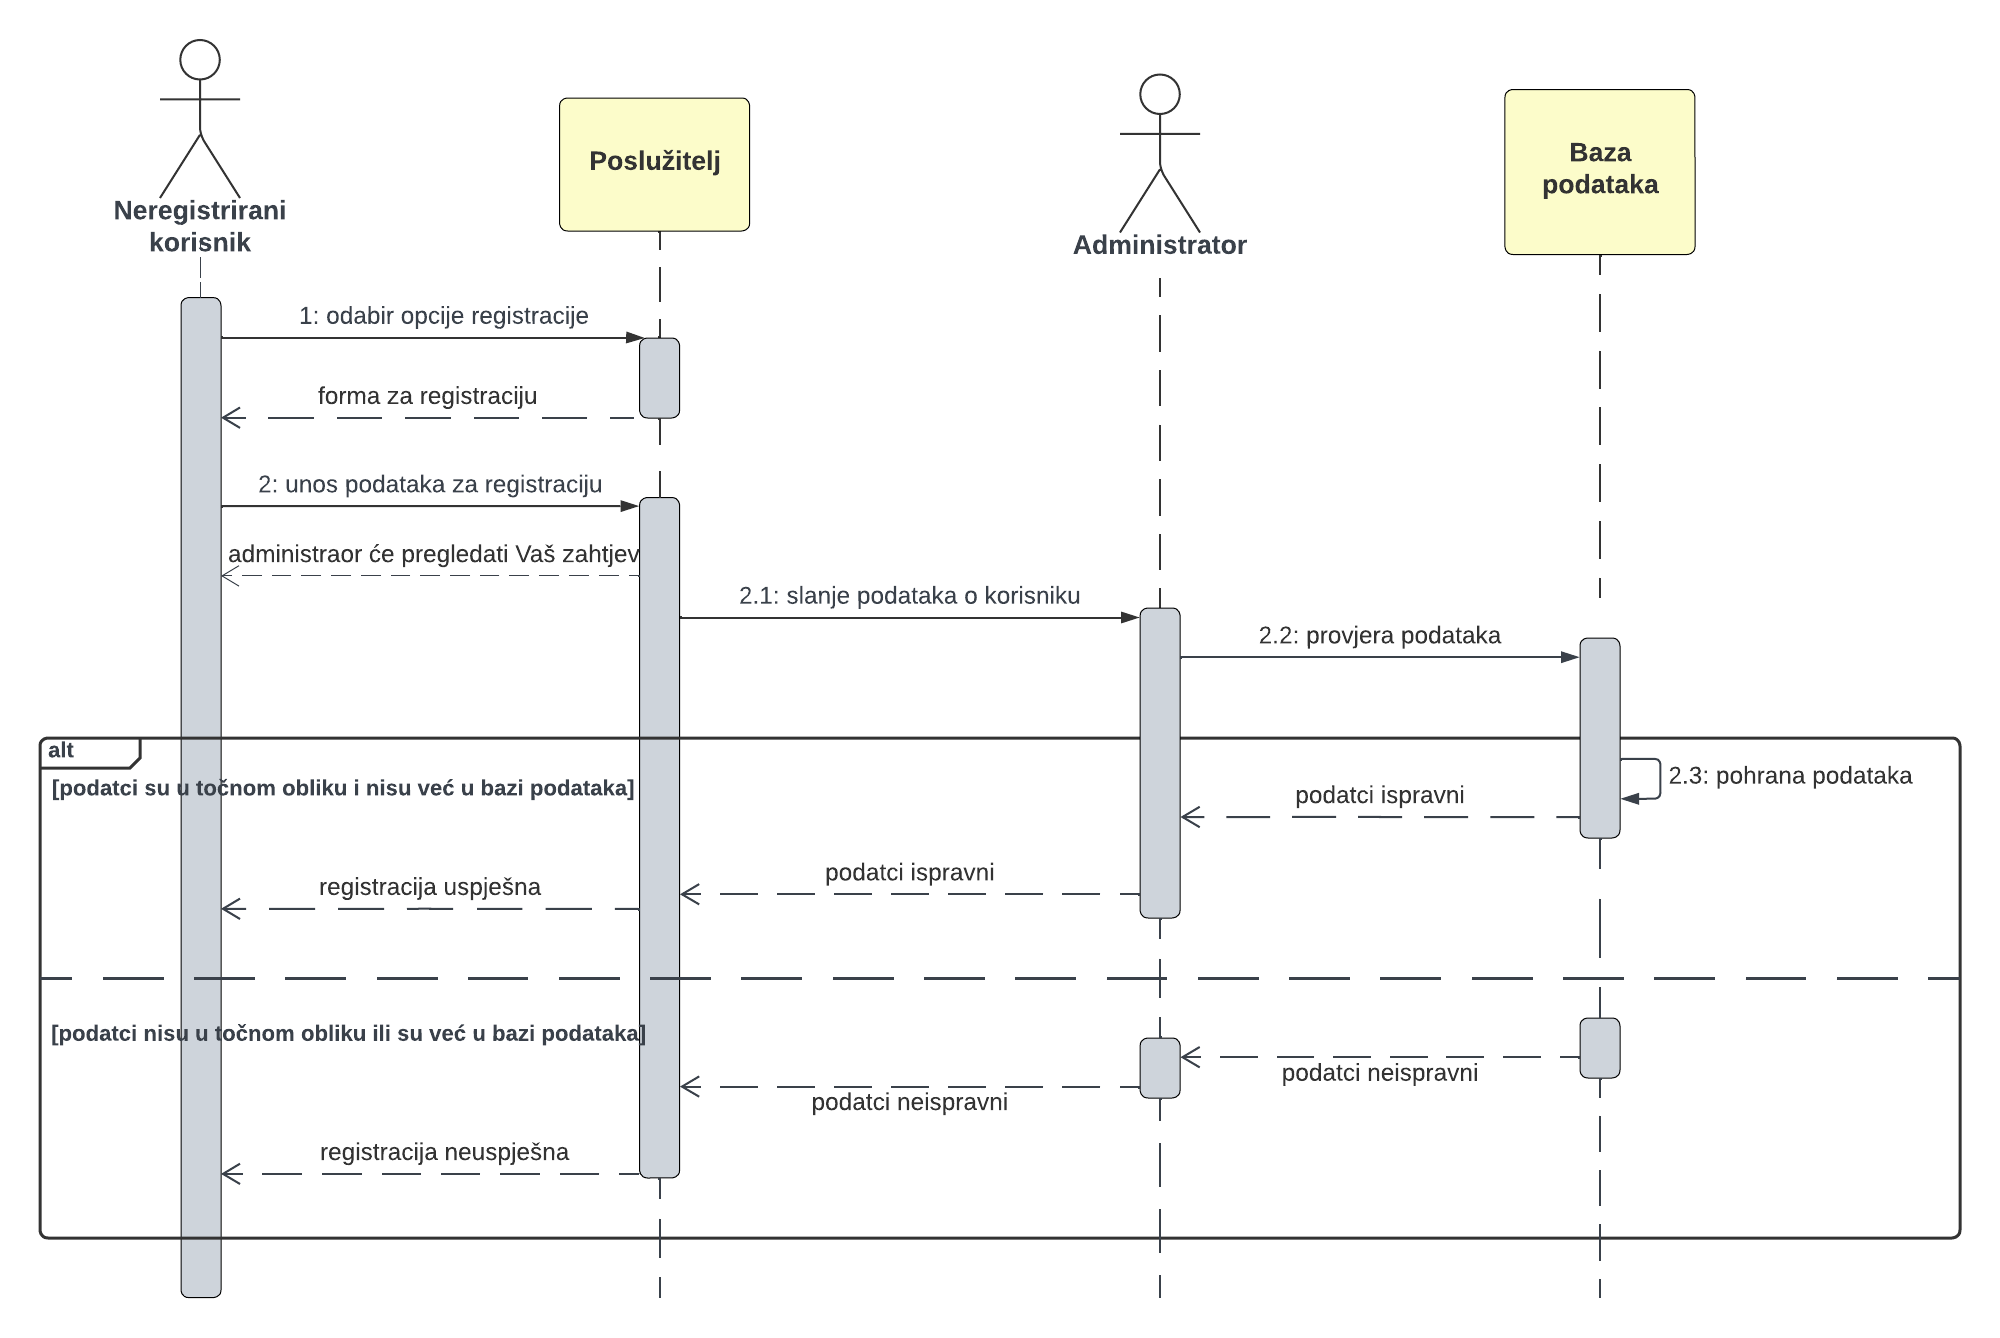
\includegraphics[width = \textwidth]{slike/sekvUC1UC3.PNG}
					\caption{Sekvencijski dijagram obrazaca uporabe UC1 i UC3}
					\label{fig:enter-label}
				\end{figure}
				\eject
				
				\textbf{Obrazac uporabe UC6 – Dodavanje objave knjige}\\\\
				Ponuditelj odabire opciju za dodavanje nove objave. Poslužitelj mu otvara stranicu za dodavanje knjiga. Nakon što ponuditelj unese sve potrebne podatke u dobrom obliku, naslov se dodaje u bazu podataka te javlja ponuditelju da je knjiga uspješno dodana. Ako želi, ponuditelj može dodati primjerke tog naslova.\\
				
				\begin{figure}[h]
					\centering
					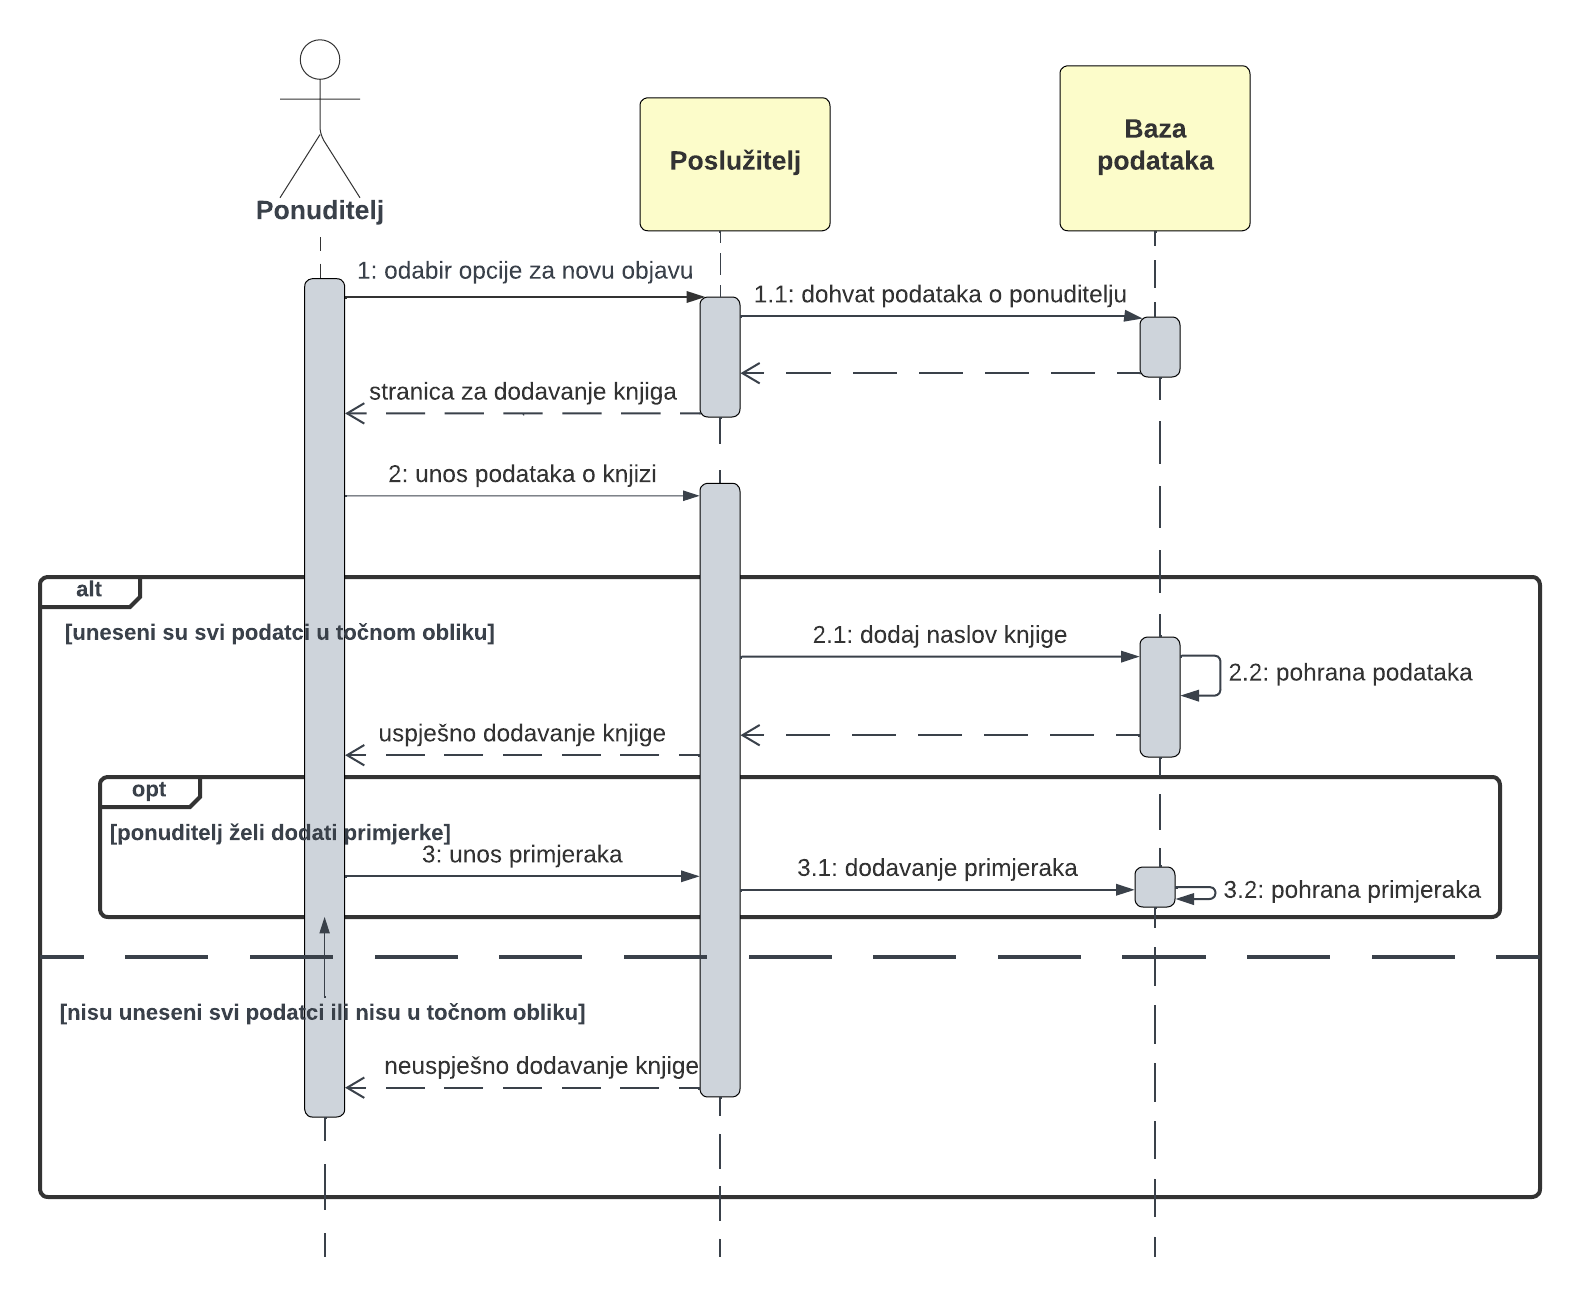
\includegraphics[width = \textwidth]{slike/sekvUC8.PNG}
					\caption{Sekvencijski dijagram obrasca uporabe UC8}
					\label{fig:enter-label}
				\end{figure}
				\eject
				
				\textbf{Obrazac uporabe UC14 - Detaljna pretraga objava knjiga i UC9 - pregled objave}\\\\
				Neregistrirani korisnik odabire opciju pretraživanja objava, a poslužitelj mu vraća formu za pretragu. Korisnik unosi potrebne podatke koje poslužitelj uspoređuje s onima u bazi podataka. Ako postoji barem jedna takva knjiga, poslužitelj prikazuje listu knjiga koje odgovaraju podatcima koje je unio neregistrirani korisnik. Ako korisnik to želi, može detaljnije pregledati podatke o nekoj objavi knjige klikom na tu objavu. Poslužitelj dohvaća potrebne podatke iz baze i prikazuje ih korisniku.\\
				
				\begin{figure}[htbp]
					\centering
					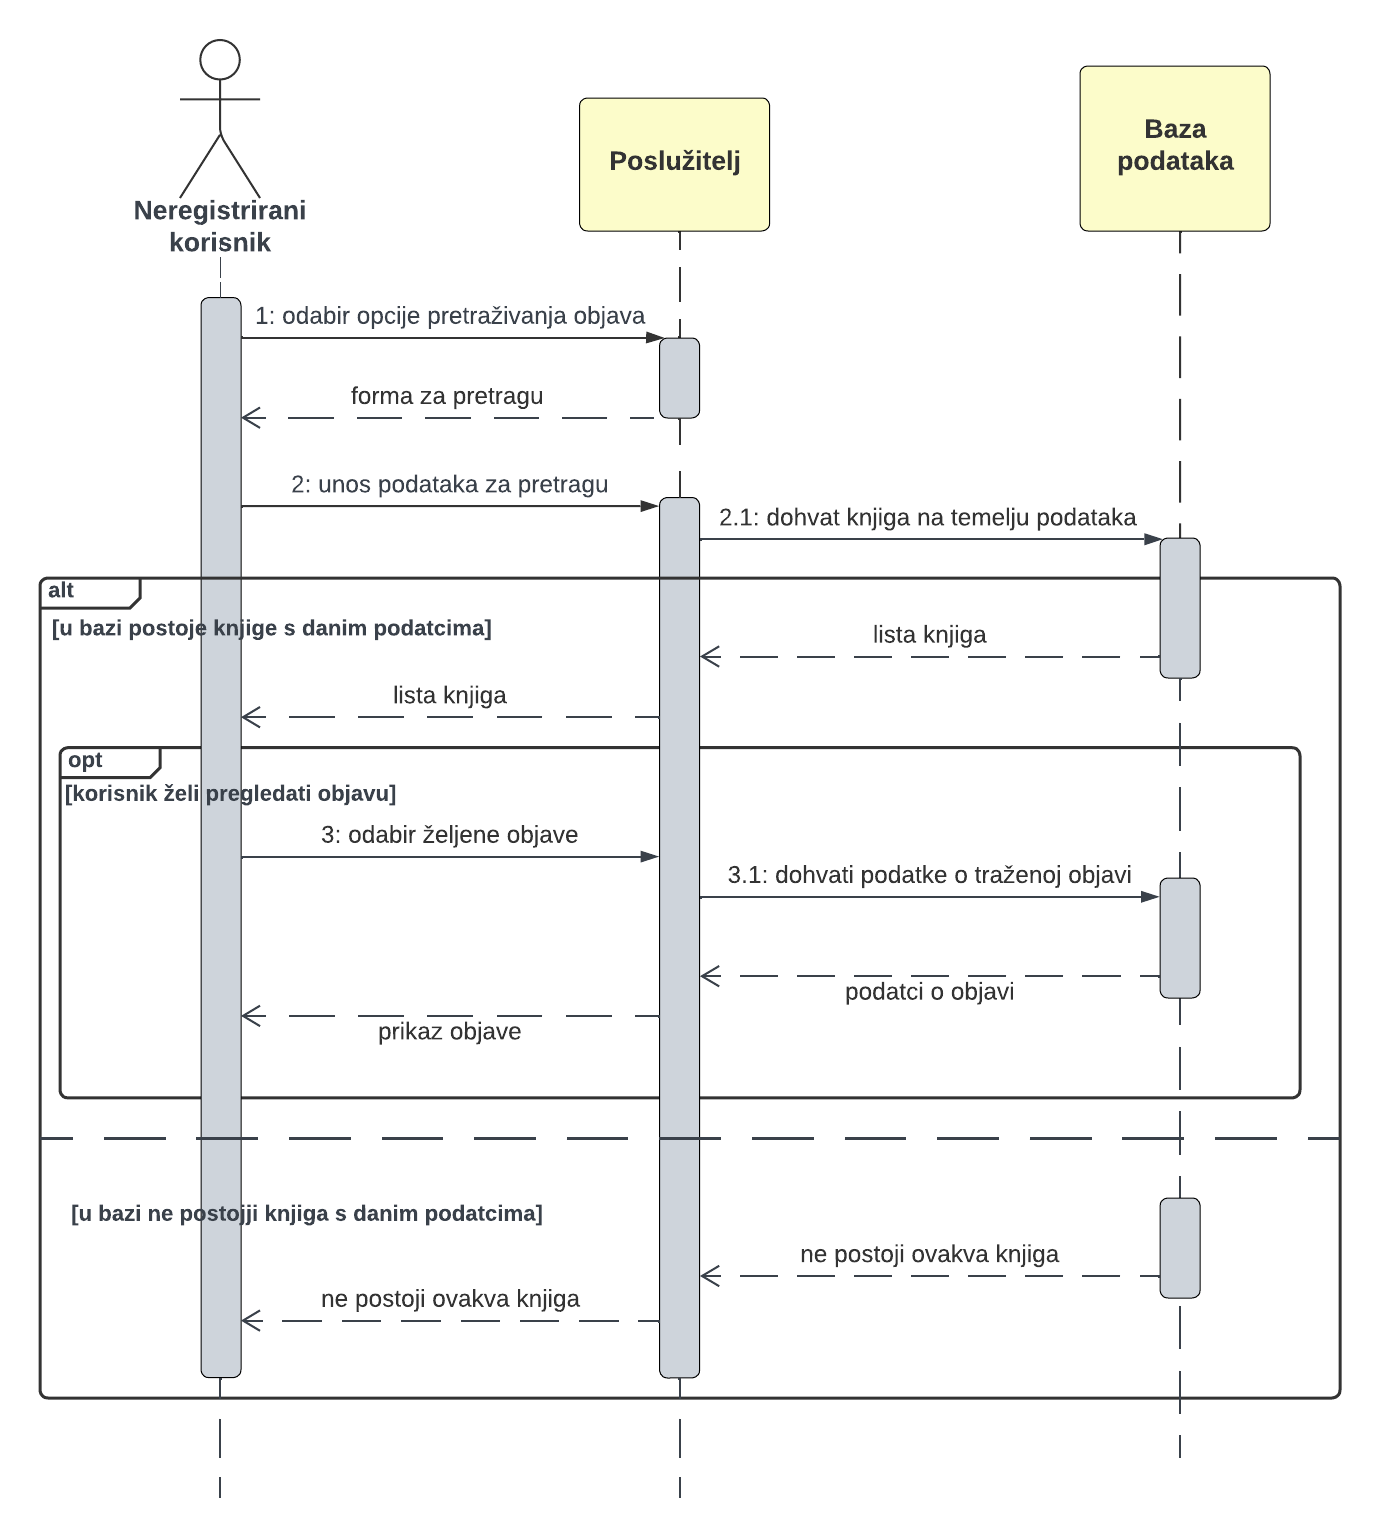
\includegraphics[width = \textwidth]{slike/sekvUC16.PNG}
					\caption{Sekvencijski dijagram obrazaca uporabe UC11 i UC16}
					\label{fig:enter-label}
				\end{figure}
				\eject
	
	
		\section{Ostali zahtjevi}
		
			
			 \begin{packed_item}
			 
			 \item Korisničko sučelje mora biti responzivno, dakle prilagođeno i stolnim računalima i mobilnim uređajima.
			 
			 \item Osnovne funkcionalnosti moraju biti jasno vidljive i dostupne u nekoliko klikova.
			 
			 \item Vrijeme odziva na obične naredbe treba biti manje od sekundu, a upiti bazi podataka moraju primiti odgovor za manje od pet sekundi.
			 
			 \item Web aplikacija mora biti implementirana objektno-orijentiranim jezikom.
			 
			 \item Sustav mora podržavati istovremen rad više korisnika.
			 
			 \item Cijene moraju biti u eurima, ali neka bude prikazana cijena i u kunama.
			 
			 \item Sustav mora informirati korisnika o nepravilnom korištenju.
			 
			 \item Mora biti omogućen pristup sustavu preko HTTPS-a.
			 
			 \item Veza s bazom podataka mora biti sigurna.
			 
			 	
			 \end{packed_item}
			 
			 
			
			 
			 